\documentclass[12pt,a4paper]{article}
\usepackage[utf8]{inputenc}
\usepackage[spanish]{babel}
\usepackage{graphicx}
\usepackage{listings}
\usepackage{xcolor}
\usepackage{hyperref}
\usepackage{float}
\usepackage[margin=2.5cm]{geometry}

% Configuración de colores para códigos
\definecolor{codegreen}{rgb}{0,0.6,0}
\definecolor{codegray}{rgb}{0.5,0.5,0.5}
\definecolor{codepurple}{rgb}{0.58,0,0.82}
\definecolor{backcolour}{rgb}{0.95,0.95,0.92}

\lstdefinestyle{mystyle}{
    backgroundcolor=\color{backcolour},   
    commentstyle=\color{codegreen},
    keywordstyle=\color{magenta},
    numberstyle=\tiny\color{codegray},
    stringstyle=\color{codepurple},
    basicstyle=\ttfamily\footnotesize,
    breakatwhitespace=false,         
    breaklines=true,                 
    captionpos=b,                    
    keepspaces=true,                 
    numbers=left,                    
    numbersep=5pt,                  
    showspaces=false,                
    showstringspaces=false,
    showtabs=false,                  
    tabsize=2
}

\lstset{style=mystyle}

\begin{document}
% Portada
\begin{titlepage}
    \centering
    \vspace*{1cm}
    
\includegraphics[width=0.8\linewidth]{espe.png}\\[0.5cm]
    
    \Large \textbf{Departamento de Ciencias de la Computación}\\
    \large \textbf{Universidad de las Fuerzas Armadas - ESPE}\\[0.5cm]
    
    \Huge \textbf{Práctica de Laboratorio No. 4}\\[0.3cm]
    \Large \textbf{Exploración de Vulnerabilidades SQL Injection con SQLmap.}\\[0.8cm]
    
    \textbf{Nombres:}\\
    Yeshua Amador Chiliquinga Amaya\\
    Cesar Ignacio Loor Mercado\\[0.3cm]
    
    \textbf{Carrera / Asignatura:} Ingeniería de Software / Ingeniería de Seguridad de Software\\
    \textbf{NRC:} 23358\\
    \textbf{Nombre del profesor:} Walter Fuertes, PhD\\[0.5cm]
    
    \textbf{Fecha de presentación:} 24 de mayo del 2025\\[1cm]    
    \vfill
\end{titlepage}
% Índice de contenido

\tableofcontents
\newpage

\section{Objetivo}
Explorar las Vulnerabilidades SQL Injection (SQLi) utilizando SQLmap en un entorno virtual de red controlado.

\section{Requerimientos}
\begin{itemize}
    \item Ubuntu Desktop – Cliente con navegador para interacción manual (opcional).
    \item Ubuntu Server – Servidor web con aplicación vulnerable (p. ej., DVWA o Mutillidae) y base de datos (MySQL/MariaDB).
    \item Kali Linux – Máquina atacante con SQLmap y herramientas ofensivas.
    \item VirtualBox o cualquier otra herramienta de virtualización para gestionar las máquinas virtuales.
    \item Acceso a Internet para descarga de herramientas y recursos.
    \item OWASP top ten attacks: una lista de los 10 principales ataques de ciberseguridad a las aplicaciones web y una guía metodológica que proporciona herramientas, documentación y estándares que ayuden a desarrolladores, organizaciones y profesionales de seguridad a crear aplicaciones web seguras.
\end{itemize}

\section{Objetivos de Aprendizaje}
\begin{itemize}
    \item Aprender a identificar y explotar vulnerabilidades de inyección SQL utilizando herramientas automatizadas como SQLmap.
    \item Familiarizarse con el análisis de aplicaciones web vulnerables a ataques SQL Injection.
    \item Comprender las implicaciones de la inyección SQL para la seguridad de las bases de datos y cómo prevenirla.
    \item Desarrollar la capacidad de implementar pruebas de penetración y análisis de seguridad en aplicaciones web.
    \item Comprender el alcance de OWASP.
\end{itemize}

\section{Marco Teórico}
\subsection{Inyección SQL (SQL Injection)}
La inyección SQL es una técnica de ataque cibernético que permite a un atacante ejecutar código SQL malicioso en una aplicación web. Este ataque se produce cuando una aplicación web no valida adecuadamente los datos introducidos por el usuario, permitiendo que estos datos se incluyan directamente en una consulta SQL. Esto puede permitir que un atacante obtenga acceso no autorizado a bases de datos, manipule datos y ejecute comandos maliciosos.

\subsection{OWASP}
(Open Worldwide Application Security Project) es una comunidad abierta y sin fines de lucro que se dedica a mejorar la seguridad del software. Su propósito principal es proporcionar herramientas, documentación y estándares que ayuden a desarrolladores, organizaciones y profesionales de seguridad a crear aplicaciones seguras. Uno de sus proyectos más conocidos es el OWASP Top Ten, una lista de las diez principales vulnerabilidades de seguridad en aplicaciones web, actualizada periódicamente según las amenazas más críticas observadas en la industria (OWASP, 2021).

\subsection{SQLmap}
Es una herramienta de prueba de penetración automatizada de código abierto diseñada para detectar y explotar vulnerabilidades de inyección SQL en aplicaciones web. SQLmap realiza pruebas de seguridad a sitios web con el objetivo de identificar debilidades y simula ataques para demostrar cómo un atacante podría comprometer la seguridad de una base de datos.

\section{Desarrollo de la Práctica}
\subsection{1. Instalación de SQLmap}
Para instalar SQLmap en la máquina local, ejecutar los siguientes comandos:

\begin{lstlisting}[language=bash, caption=Instalación de SQLmap en Linux]
sudo apt-get update
sudo apt-get install sqlmap
\end{lstlisting}

\subsection{2. Exploración de un Sitio Web Vulnerable}
Se utilizó un entorno de laboratorio con una aplicación web vulnerable a inyección SQL. Se configuró el entorno con Damn Vulnerable Web Application (DVWA):

\begin{enumerate}
    \item Acceder a DVWA desde el navegador: \texttt{http://[IP-SERVER]/DVWA/}
    \item Iniciar sesión con las credenciales por defecto (usuario: admin, contraseña: password)
    \item Configurar el nivel de seguridad en "Low" para habilitar la vulnerabilidad de inyección SQL
    \item Acceder a la página de "SQL Injection"
    \item Probar URL vulnerable: \texttt{http://[IP]/DVWA/vulnerabilities/sqli/?id=1\&Submit=Submit}
\end{enumerate}

\begin{figure}[H]
    \centering
    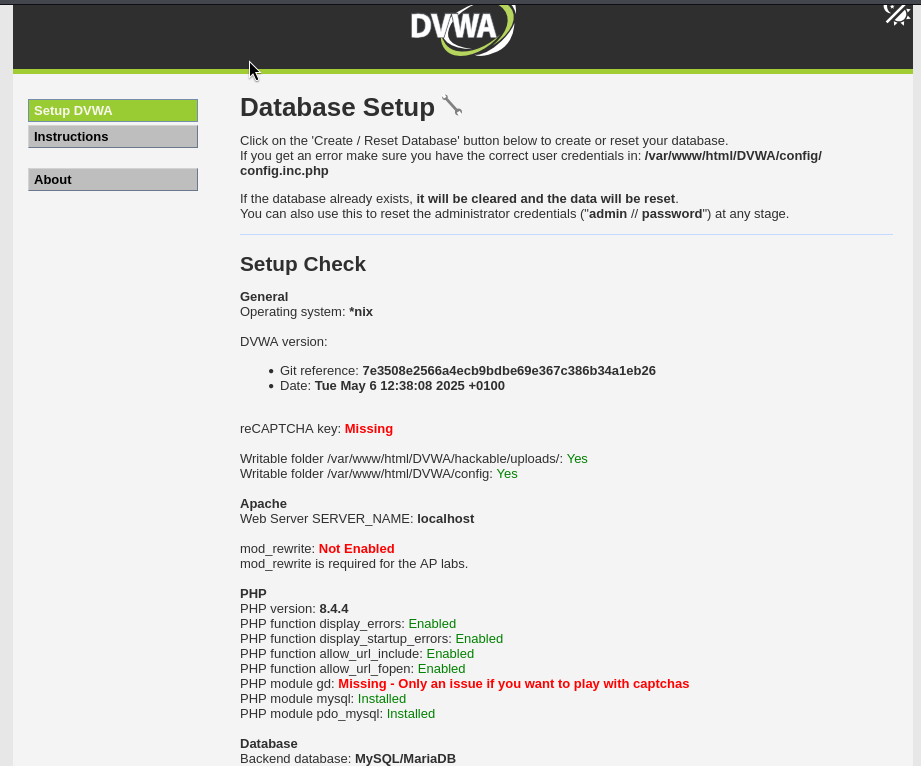
\includegraphics[width=0.9\textwidth]{dvwa_page.png}
    \caption{Página principal de DVWA}
    \label{fig:dvwa}
\end{figure}

\subsection{3. Uso de SQLmap}
Para detectar vulnerabilidades en el sitio web, se utilizó el siguiente comando:

\begin{figure}[H]
    \centering
    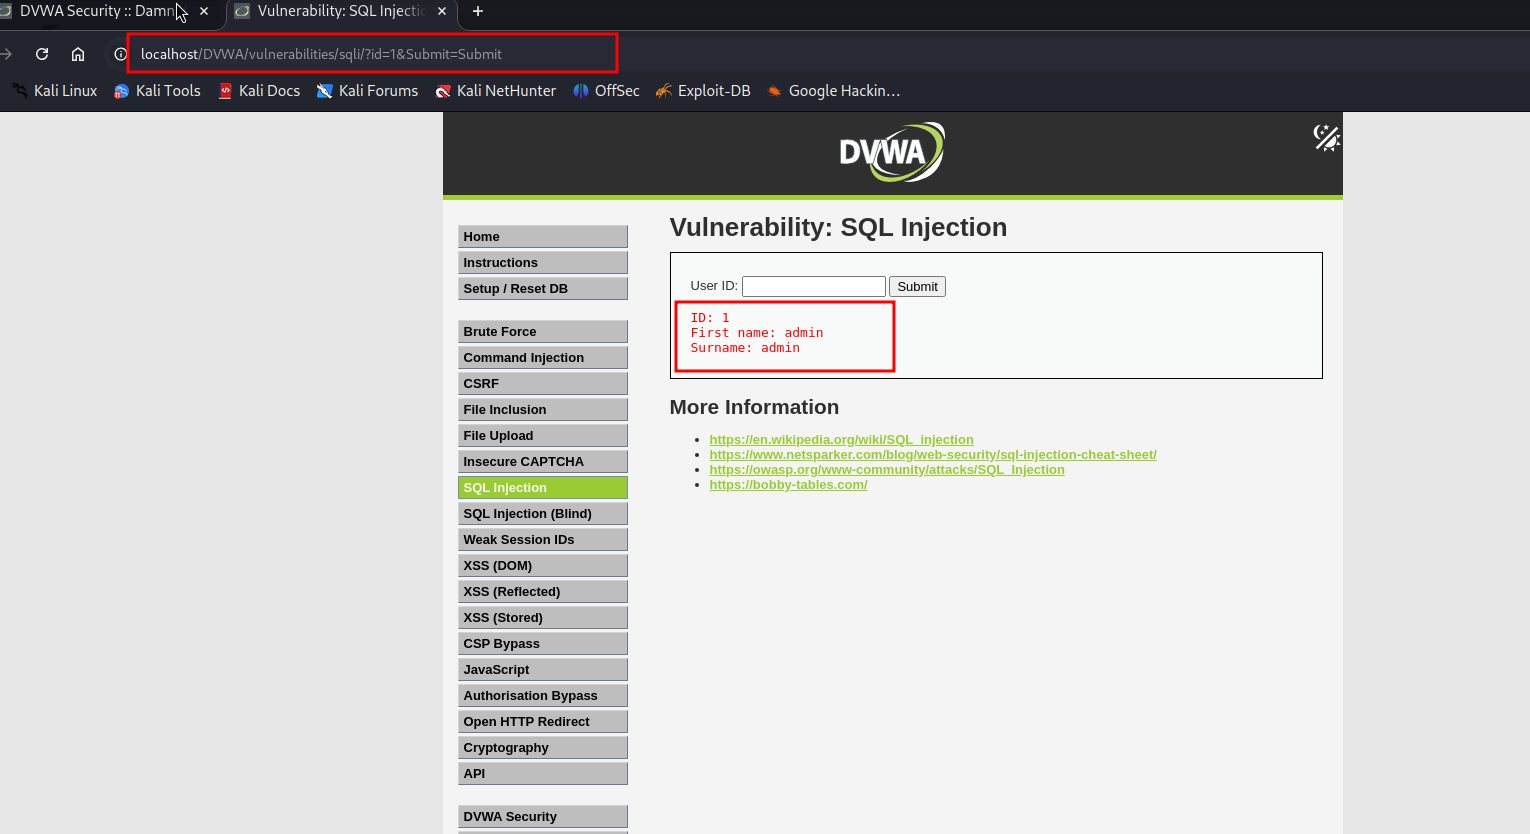
\includegraphics[width=0.9\textwidth]{id_1.png}
    \caption{Ejemplo de inyección SQL directa en la URL}
    \label{fig:id_1}
\end{figure}

\begin{lstlisting}[language=bash, caption=Uso básico de SQLmap]
sqlmap -u "http://localhost/dvwa/vulnerabilities/sqli/?id=1&Submit=Submit" --batch --threads=10
\end{lstlisting}

\begin{description}
    \item[-u] La URL del sitio web vulnerable
    \item[--batch] Ejecuta SQLmap sin pedir confirmaciones al usuario
    \item[--threads=10] Aumenta la velocidad de las pruebas utilizando 10 hilos concurrentes
\end{description}

\begin{figure}[H]
    \centering
    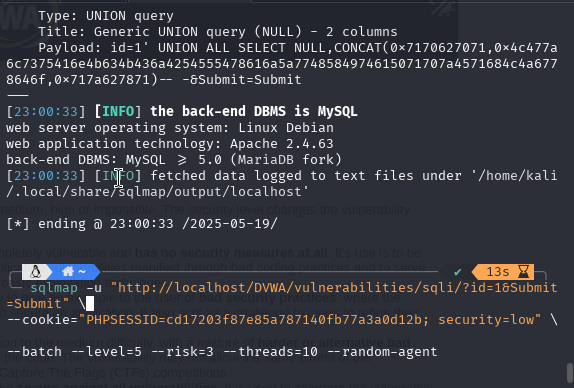
\includegraphics[width=0.9\textwidth]{sqlmap_threads.png}
    \caption{Ejecución de SQLmap con múltiples hilos}
    \label{fig:sqlmap_threads}
\end{figure}

\subsection{4. Explotación de la Vulnerabilidad}
Una vez identificada la vulnerabilidad, se procedió a obtener información de la base de datos:

\begin{figure}[H]
    \centering
    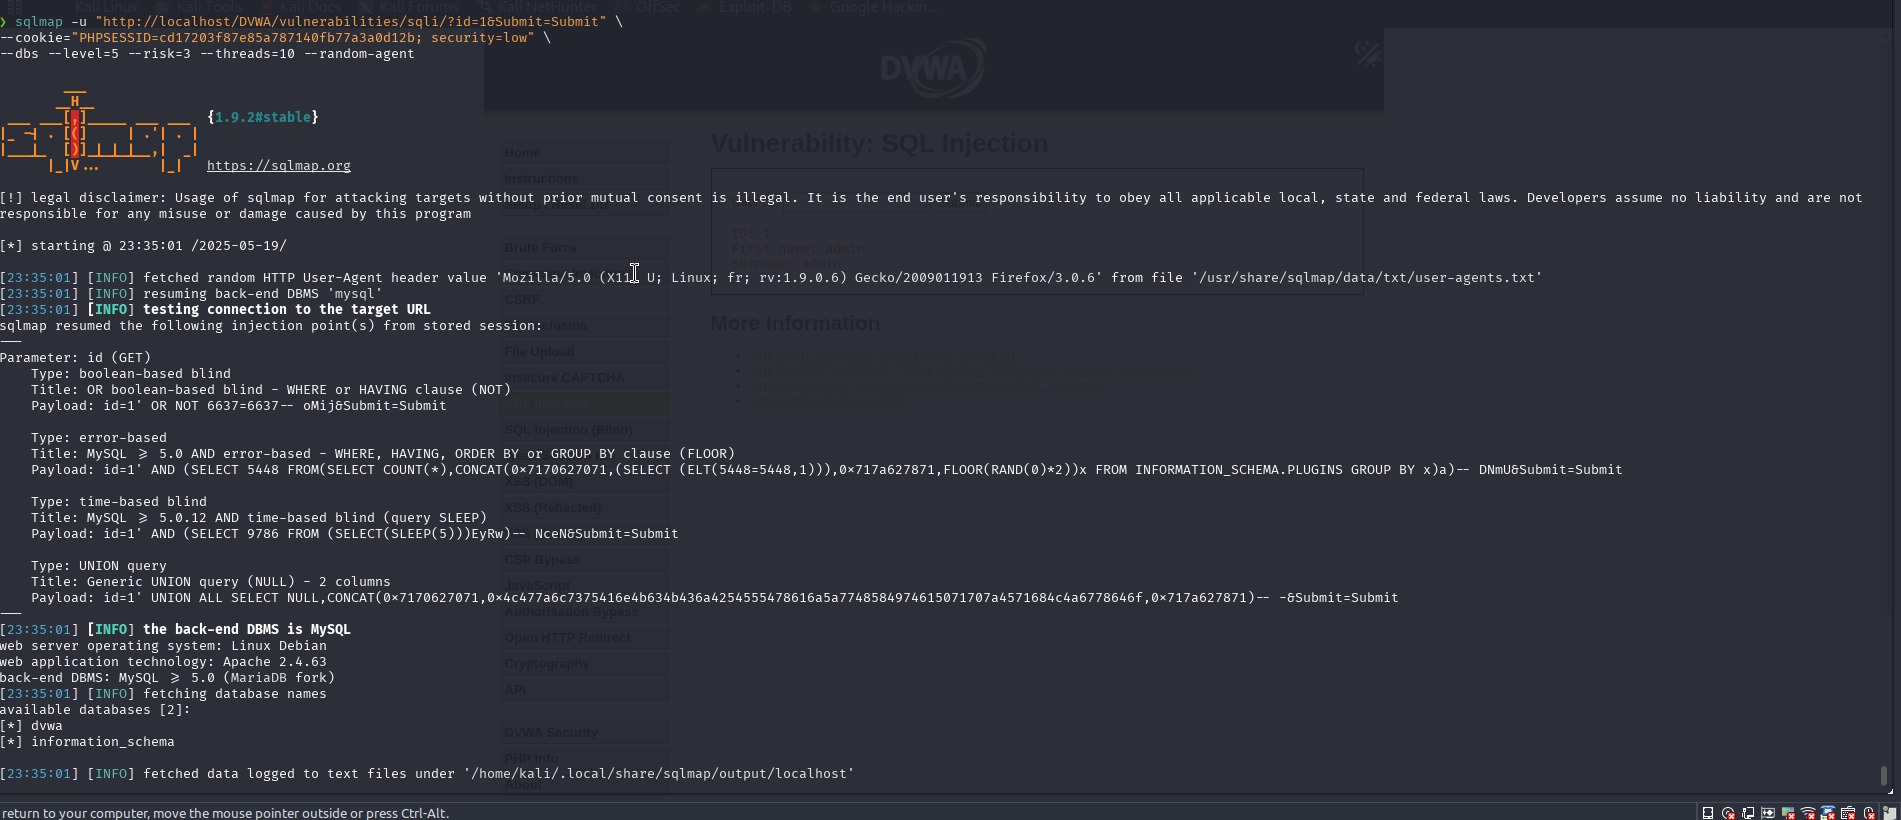
\includegraphics[width=0.9\textwidth]{database.png}
    \caption{Estructura de la base de datos vulnerable}
    \label{fig:database}
\end{figure}

\begin{lstlisting}[language=bash, caption=Obtención de bases de datos]
sqlmap -u "http://localhost/dvwa/vulnerabilities/sqli/?id=1&Submit=Submit" --dbs
\end{lstlisting}

\begin{figure}[H]
    \centering
    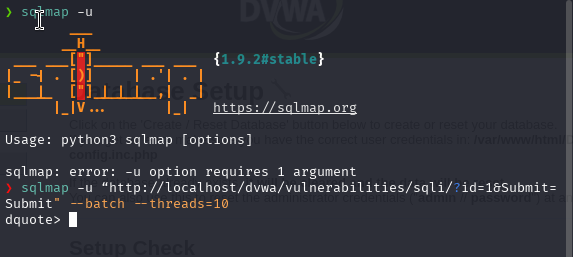
\includegraphics[width=0.9\textwidth]{sqlmap_u.png}
    \caption{Resultado de la exploración con SQLmap}
    \label{fig:sqlmap_u}
\end{figure}

\subsection{5. Simulación de SQL Injection en un sitio web desarrollado}
Se creó una base de datos vulnerable y una aplicación web para demostrar la inyección SQL:

\begin{lstlisting}[language=sql, caption=Creación de base de datos vulnerable]
CREATE DATABASE estudianteDB;
USE estudianteDB;
CREATE TABLE empleados (
  id INT AUTO_INCREMENT PRIMARY KEY,
  nombre VARCHAR(50),
  cargo VARCHAR(50)
);
INSERT INTO empleados (nombre, cargo) VALUES ('Ana', 'Analista'), ('Luis', 'Desarrollador');
\end{lstlisting}

\begin{figure}[H]
    \centering
    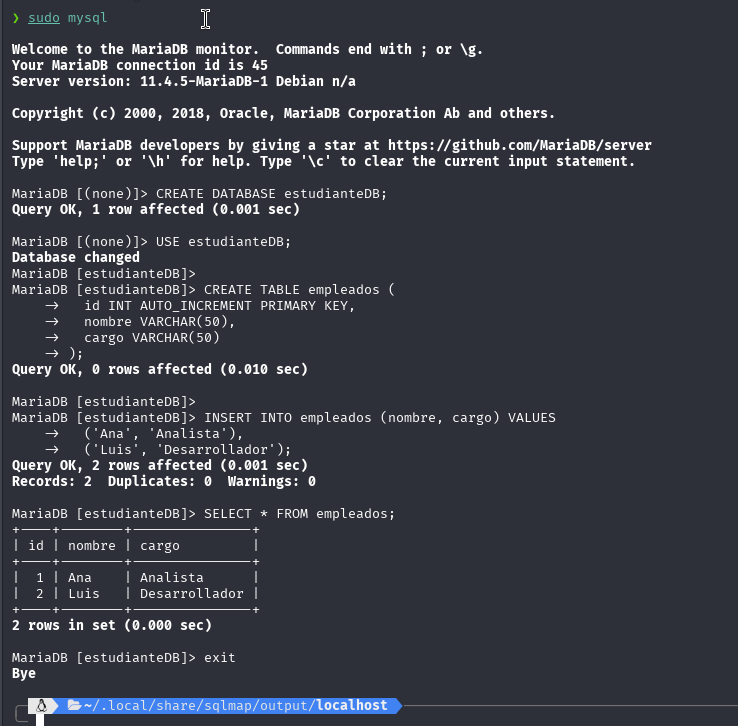
\includegraphics[width=0.9\textwidth]{create_database.png}
    \caption{Creación de la base de datos vulnerable}
    \label{fig:create_db}
\end{figure}

Se desarrolló una aplicación web vulnerable en PHP:

\begin{lstlisting}[language=php, caption=Aplicación web vulnerable]
<?php
$conn = mysqli_connect("localhost", "root", "", "estudianteDB");
$id = $_GET['id'];
$sql = "SELECT * FROM empleados WHERE id = $id";
$result = mysqli_query($conn, $sql);

while($row = mysqli_fetch_assoc($result)) {
    echo "Nombre: " . $row['nombre'] . " - Cargo: " . $row['cargo'] . "<br>";
}
?>
\end{lstlisting}

\begin{figure}[H]
    \centering
    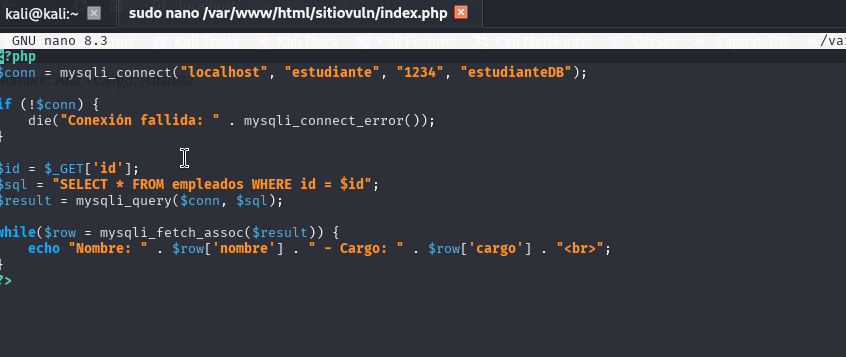
\includegraphics[width=0.9\textwidth]{html.png}
    \caption{Código HTML de la página vulnerable}
    \label{fig:html}
\end{figure}

\subsection{6. Prevención de SQL Injection}
Para prevenir vulnerabilidades de inyección SQL, se recomienda:

\begin{itemize}
    \item Validación y sanitización de las entradas del usuario
    \item Uso de consultas preparadas (prepared statements)
    \item Implementación de control de acceso adecuado en la base de datos
    \item Uso de ORM (Object Relational Mapping) que automáticamente previene inyecciones SQL
\end{itemize}

\section{Conclusión}

\begin{figure}[H]
    \centering
    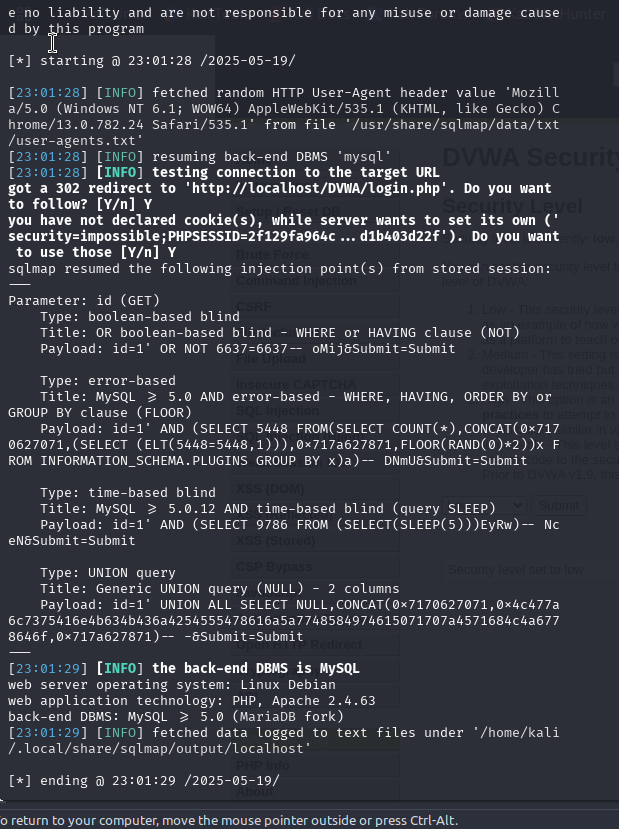
\includegraphics[width=0.9\textwidth]{cookie.png}
    \caption{Información de cookies en la aplicación vulnerable}
    \label{fig:cookie}
\end{figure}

Esta práctica permitió comprender cómo funcionan los ataques de inyección SQL y cómo pueden ser detectados y explotados utilizando herramientas como SQLmap. Se pudo evidenciar la importancia de implementar buenas prácticas de desarrollo para proteger las aplicaciones web de estos ataques, como el uso de consultas preparadas y la validación de entradas.

\begin{figure}[H]
    \centering
    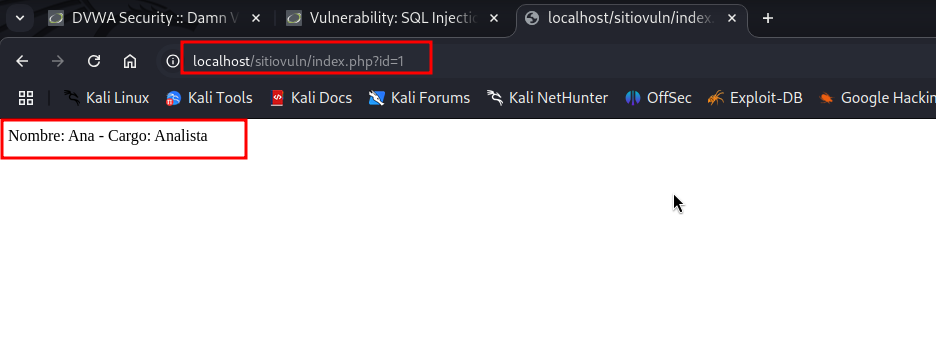
\includegraphics[width=0.9\textwidth]{pagina_estudiante.png}
    \caption{Página del estudiante vulnerable}
    \label{fig:pagina_estudiante}
\end{figure}

\section{Referencias bibliográficas}
\begin{itemize}
    \item OWASP. (2021). OWASP Top Ten. Recuperado de https://owasp.org/www-project-top-ten/
    \item SQLmap Project. (2023). SQLmap: Automatic SQL injection and database takeover tool. Recuperado de http://sqlmap.org/
    \item PortSwigger. (2023). SQL Injection. Recuperado de https://portswigger.net/web-security/sql-injection
\end{itemize}
\end{document}